% answers.tex —— 1977 年·浙江卷 · 参考答案与详细解析片段
% 由 tools/generate_projects.py 依来源总账自 1977/1977_数学真题_浙江_试题.md + 1977/1977_数学真题_浙江_解析正文.md + 1977/1977_数学真题_浙江_答案要点.md 生成，勿手改（改源 MD 后重跑）


\begin{gktip}
固定源是题面与解答连续出现的扫描材料。下文逐题对照源解答并重新计算关键结论；原卷大题的汉数字编号已按题库规范重排为阿拉伯数字 1—7，大题内阿拉伯数字小项重排为（1）（2）（3）。参考题 2 源解答末行合并对数时把 $(x+3)$ 的指数印作 $2$，与前一行系数 $3$ 矛盾，系排印错误，详见该题源注。
\end{gktip}

\begin{answer}
\gksolhead{1}{}

\textbf{题目}：

计算：

（1） $\sqrt[6]{8^5}\div\sqrt{8}\times\sqrt[3]{8}\div\left(\dfrac18\right)^0$（本题 5 分）。

（2） $\dfrac{\lg 4+\lg 25-\lg 10}{\lg\sqrt{1000}}$（本题 5 分）。

（3） $\dfrac{1}{100\times101}+\dfrac{1}{101\times102}+\dfrac{1}{102\times103}+\cdots+\dfrac{1}{149\times150}$（本题 5 分）。

\Needspace{4\baselineskip}
\textbf{解析}

\gksubpart{（1）}

\Needspace{5\baselineskip}
由 $8=2^3$ 得

\nopagebreak[4]
\[
\sqrt[6]{8^5}=8^{5/6}=2^{15/6}=2^{5/2}=4\sqrt2,
\qquad
\sqrt8=2\sqrt2,
\qquad
\sqrt[3]{8}=2,
\]

\Needspace{5\baselineskip}
且 $\left(\dfrac18\right)^0=1$。于是

\nopagebreak[4]
\[
\sqrt[6]{8^5}\div\sqrt8\times\sqrt[3]{8}\div\left(\frac18\right)^0
=4\sqrt2\div2\sqrt2\times2\div1=4.
\]

\gksubpart{（2）}

\Needspace{5\baselineskip}
分子 $\lg4+\lg25-\lg10=\lg\dfrac{4\times25}{10}=\lg10=1$，分母 $\lg\sqrt{1000}=\lg10^{\frac32}=\dfrac32$，所以

\nopagebreak[4]
\[
\frac{\lg4+\lg25-\lg10}{\lg\sqrt{1000}}=\frac{1}{\frac32}=\frac23.
\]

\gksubpart{（3）}

\Needspace{5\baselineskip}
用裂项 $\dfrac{1}{k(k+1)}=\dfrac1k-\dfrac{1}{k+1}$，从 $k=100$ 到 $k=149$ 逐项相消，只剩首尾两项：

\nopagebreak[4]
\[
\frac{1}{100\times101}+\frac{1}{101\times102}+\cdots+\frac{1}{149\times150}
=\frac1{100}-\frac1{150}
=\frac{50}{15000}=\frac1{300}.
\]

\gkanswer{答案（1）：$4$。}

\gkanswer{答案（2）：$\dfrac23$。}

\gkanswer{答案（3）：$\dfrac1{300}$。}

\end{answer}
\begin{answer}
\gksolhead{2}{}

\textbf{题目}：

（1） 已知 $\operatorname{tg}\alpha=\sqrt2$，求 $\dfrac{\cos\alpha+\sin\alpha}{\cos\alpha-\sin\alpha}$ 的值（本题 5 分）。

（2） 求 $\sin^262^\circ+\operatorname{tg}54^\circ\cdot\operatorname{tg}45^\circ\cdot\operatorname{tg}36^\circ+\sin^228^\circ$ 的值（本题 5 分）。

（3） 某生产队要建一个贮粮用的“土圆仓”，如果土圆仓下部圆柱和上部圆锥的底面半径都是 1.5 米，高分别是 3 米和 0.6 米，计算它的容积（$\pi\approx3.14$，精确到 0.1 立方米）（本题 8 分）。

\begin{gktip}
原源 PDF 第 1 页右下附有土圆仓（下部圆柱、上部圆锥）示意图；LaTeX 版按源图重绘。
\end{gktip}
\nopagebreak[4]
\begin{center}% 1977 年浙江卷第 2(3) 题：贮粮“土圆仓”，下部圆柱、上部圆锥，
% 轴虚线自锥顶贯穿到底面圆心，标注圆锥高 0.6 米、圆柱高 3 米、底面半径 r=1.5 米（按源卷第 1 页布局）
\begin{tikzpicture}[scale=0.9]
  % 圆柱轮廓
  \draw[thick] (-1.6,0)--(-1.6,3);
  \draw[thick] (1.6,0)--(1.6,3);
  % 底面椭圆：后半虚线、前半实线
  \draw[dashed] (1.6,0) arc (0:180:1.6 and 0.42);
  \draw[thick] (1.6,0) arc (0:-180:1.6 and 0.42);
  % 顶面椭圆（即圆锥底面）：后半虚线、前半实线
  \draw[dashed] (1.6,3) arc (0:180:1.6 and 0.42);
  \draw[thick] (1.6,3) arc (0:-180:1.6 and 0.42);
  % 圆锥两条母线
  \draw[thick] (-1.6,3)--(0,4.15)--(1.6,3);
  % 轴线与半径（虚线）
  \draw[dashed] (0,4.15)--(0,0);
  \draw[dashed] (0,3)--(1.6,3);
  \draw[dashed] (0,0)--(1.6,0);
  % 标注
  \node[rotate=90] at (-0.34,3.6) {$0.6$ 米};
  \node[rotate=90] at (-0.34,1.5) {$3$ 米};
  \node at (0.78,-0.4) {$r=1.5$ 米};
\end{tikzpicture}
\end{center}
\nopagebreak[4]
\Needspace{4\baselineskip}
\textbf{解析}

\gksubpart{（1）}

\Needspace{5\baselineskip}
$\tan\alpha$ 有意义要求 $\cos\alpha\ne0$，分子、分母同除以 $\cos\alpha$：

\nopagebreak[4]
\[
\frac{\cos\alpha+\sin\alpha}{\cos\alpha-\sin\alpha}
=\frac{1+\tan\alpha}{1-\tan\alpha}
=\frac{1+\sqrt2}{1-\sqrt2}.
\]

\Needspace{5\baselineskip}
分母有理化（分子分母同乘 $1+\sqrt2$）：

\nopagebreak[4]
\[
\frac{1+\sqrt2}{1-\sqrt2}
=\frac{(1+\sqrt2)^2}{(1-\sqrt2)(1+\sqrt2)}
=\frac{3+2\sqrt2}{-1}
=-3-2\sqrt2.
\]

\gksubpart{（2）}

\Needspace{5\baselineskip}
$62^\circ$ 与 $28^\circ$ 互余，故 $\sin28^\circ=\cos62^\circ$；$54^\circ$ 与 $36^\circ$ 互余，故 $\tan36^\circ=\cot54^\circ$。于是

\nopagebreak[4]
\[
\begin{gathered}
\sin^262^\circ+\tan54^\circ\cdot\tan45^\circ\cdot\tan36^\circ+\sin^228^\circ\\
=\underbrace{\left(\sin^262^\circ+\cos^262^\circ\right)}_{=1}
+\underbrace{\left(\tan54^\circ\cdot\cot54^\circ\right)}_{=1}\cdot\tan45^\circ
=1+1=2.
\end{gathered}
\]

\gksubpart{（3）}

\Needspace{5\baselineskip}
设圆柱的高为 $h_1=3$ 米、圆锥的高为 $h_2=0.6$ 米，底面半径 $r=1.5$ 米。粮仓容积为圆柱与圆锥两部分之和：

\nopagebreak[4]
\[
V=\pi r^2h_1+\frac13\pi r^2h_2
=\pi r^2\left(h_1+\frac13h_2\right).
\]

\Needspace{5\baselineskip}
取 $\pi\approx3.14$：

\nopagebreak[4]
\[
V\approx3.14\times1.5^2\times\left(3+\frac13\times0.6\right)
=3.14\times2.25\times3.2
=22.608\approx22.6\ \text{\text{立方米}}.
\]
\nopagebreak[4]
\begin{center}% 1977 年浙江卷第 2(3) 题：贮粮“土圆仓”，下部圆柱、上部圆锥，
% 轴虚线自锥顶贯穿到底面圆心，标注圆锥高 0.6 米、圆柱高 3 米、底面半径 r=1.5 米（按源卷第 1 页布局）
\begin{tikzpicture}[scale=0.9]
  % 圆柱轮廓
  \draw[thick] (-1.6,0)--(-1.6,3);
  \draw[thick] (1.6,0)--(1.6,3);
  % 底面椭圆：后半虚线、前半实线
  \draw[dashed] (1.6,0) arc (0:180:1.6 and 0.42);
  \draw[thick] (1.6,0) arc (0:-180:1.6 and 0.42);
  % 顶面椭圆（即圆锥底面）：后半虚线、前半实线
  \draw[dashed] (1.6,3) arc (0:180:1.6 and 0.42);
  \draw[thick] (1.6,3) arc (0:-180:1.6 and 0.42);
  % 圆锥两条母线
  \draw[thick] (-1.6,3)--(0,4.15)--(1.6,3);
  % 轴线与半径（虚线）
  \draw[dashed] (0,4.15)--(0,0);
  \draw[dashed] (0,3)--(1.6,3);
  \draw[dashed] (0,0)--(1.6,0);
  % 标注
  \node[rotate=90] at (-0.34,3.6) {$0.6$ 米};
  \node[rotate=90] at (-0.34,1.5) {$3$ 米};
  \node at (0.78,-0.4) {$r=1.5$ 米};
\end{tikzpicture}
\end{center}
\nopagebreak[4]
\gkanswer{答案（1）：$-3-2\sqrt2$。}

\gkanswer{答案（2）：$2$。}

\gkanswer{答案（3）：约 $22.6$ 立方米。}

\end{answer}
\begin{answer}
\gksolhead{3}{}

\textbf{题目}（15 分）：

求平行直线 $3x+2y-3=0$ 和 $3x+2y+2=0$ 之间的距离。

\Needspace{4\baselineskip}
\textbf{解析}

\Needspace{5\baselineskip}
点 $(1,0)$ 满足 $3\times1+2\times0-3=0$，故它是直线 $3x+2y-3=0$ 上的点。它到直线 $3x+2y+2=0$ 的距离

\nopagebreak[4]
\[
d=\frac{|3\times1+2\times0+2|}{\sqrt{3^2+2^2}}
=\frac{5}{\sqrt{13}}
=\frac{5\sqrt{13}}{13}.
\]

两条直线平行，平行线间距离处处相等，所以 $\dfrac{5\sqrt{13}}{13}$ 就是所求平行直线间的距离。

\gkanswer{答案：$\dfrac{5\sqrt{13}}{13}$。}

\end{answer}
\begin{answer}
\gksolhead{4}{}

\textbf{题目}（15 分）：

已知 $\alpha$ 和 $\beta$ 是三角形的两个内角，并且 $\alpha$ 是锐角，而 $\cos\alpha=\dfrac35$，$\sin\beta=\dfrac5{13}$，求 $\sin(\alpha+\beta)$ 的值。

\Needspace{4\baselineskip}
\textbf{解析}

$\alpha$ 为锐角且 $\cos\alpha=\dfrac35$，故 $\sin\alpha=\dfrac45$。$\sin\beta=\dfrac5{13}>0$，$\beta$ 可能是锐角也可能是钝角，故 $\cos\beta=\pm\dfrac{12}{13}$。

\Needspace{5\baselineskip}
若 $\beta$ 为锐角，$\cos\beta=\dfrac{12}{13}$，由两角和公式

\nopagebreak[4]
\[
\sin(\alpha+\beta)=\sin\alpha\cos\beta+\cos\alpha\sin\beta
=\frac45\cdot\frac{12}{13}+\frac35\cdot\frac5{13}
=\frac{48+15}{65}=\frac{63}{65}.
\]

\Needspace{5\baselineskip}
若 $\beta$ 为钝角，$\cos\beta=-\dfrac{12}{13}$，

\nopagebreak[4]
\[
\sin(\alpha+\beta)=\frac45\left(-\frac{12}{13}\right)+\frac35\cdot\frac5{13}
=\frac{-48+15}{65}=-\frac{33}{65}<0.
\]

但 $\alpha$、$\beta$ 是三角形的两个内角，$0^\circ<\alpha+\beta<180^\circ$，此时 $\sin(\alpha+\beta)$ 必为正，故 $\beta$ 为钝角的情形应舍去，$\sin(\alpha+\beta)=\dfrac{63}{65}$。

\gkanswer{答案：$\dfrac{63}{65}$。}

\end{answer}
\begin{answer}
\gksolhead{5}{}

\textbf{题目}（15 分）：

解不等式：$\log_5(x^2-2x-15)<\log_5(x+13)$。

\Needspace{4\baselineskip}
\textbf{解析}

\Needspace{5\baselineskip}
对数真数必须为正，去对数后不等式仍须成立，故 $x$ 须同时满足

\nopagebreak[4]
\[
\begin{cases}
x^2-2x-15<x+13,\\
x^2-2x-15>0,\\
x+13>0.
\end{cases}
\]

第一式即 $x^2-3x-28<0$，也就是 $(x+4)(x-7)<0$，解得 $-4<x<7$；第二式即 $(x+3)(x-5)>0$，解得 $x<-3$ 或 $x>5$；第三式解得 $x>-13$。

三个条件取交集：$x>5$ 与 $-4<x<7$ 相交得 $5<x<7$；$x<-3$ 与 $-4<x<7$、$x>-13$ 相交得 $-4<x<-3$。所以原不等式的解为 $5<x<7$ 或 $-4<x<-3$。

\gkanswer{答案：$5<x<7$ 或 $-4<x<-3$。}

\end{answer}
\begin{answer}
\gksolhead{6}{}

\textbf{题目}（10 分）：

\Needspace{5\baselineskip}
点 $O$ 为 $\triangle ABC$ 内任意一点，连接 $AO$ 并延长交 $BC$ 于点 $D$，连接 $BO$ 并延长交 $AC$ 于点 $E$，连接 $CO$ 并延长交 $AB$ 于点 $F$，则

\nopagebreak[4]
\[
\frac{OD}{AD}+\frac{OE}{BE}+\frac{OF}{CF}=1.
\]

\begin{gktip}
原源 PDF 第 3 页附有三角形、内点 $O$ 与三条延长线示意图；LaTeX 版按源图重绘。
\end{gktip}
\nopagebreak[4]
\begin{center}% 1977 年浙江卷第六题：△ABC 内一点 O，AO 延长交 BC 于 D（虚线），BO 延长交 AC 于 E、
% CO 延长交 AB 于 F（实线），OH 为 O 到 BC 的垂线段（虚线），K 为 A 的高线足，
% BC 上自左至右标 K、H、D（按源卷第 3 页布局）
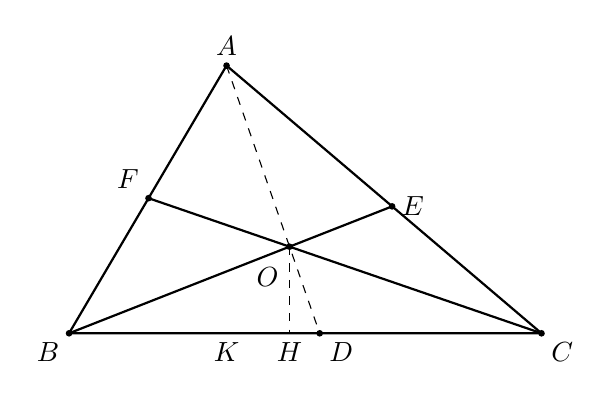
\begin{tikzpicture}[scale=1.0]
  \coordinate (A) at (2.0,3.4);
  \coordinate (B) at (0,0);
  \coordinate (C) at (6,0);
  \coordinate (O) at (2.8,1.1);
  \coordinate (D) at (3.183,0);
  \coordinate (E) at (4.103,1.612);
  \coordinate (F) at (1.009,1.716);
  \coordinate (K) at (2.0,0);
  \coordinate (H) at (2.8,0);
  \draw[thick] (A)--(B)--(C)--cycle;
  \draw[thick] (B)--(E);
  \draw[thick] (C)--(F);
  \draw[dashed] (A)--(D);
  \draw[dashed] (O)--(H);
  \fill (A) circle (1.2pt) node[above] {$A$};
  \fill (B) circle (1.2pt) node[below left] {$B$};
  \fill (C) circle (1.2pt) node[below right] {$C$};
  \fill (O) circle (1.2pt);
  \fill (D) circle (1.2pt) node[below right] {$D$};
  \fill (E) circle (1.2pt) node[right] {$E$};
  \fill (F) circle (1.2pt) node[above left] {$F$};
  \node[below] at (K) {$K$};
  \node[below] at (H) {$H$};
  \node at (2.52,0.72) {$O$};
\end{tikzpicture}
\end{center}
\nopagebreak[4]
\Needspace{4\baselineskip}
\textbf{解析}
\nopagebreak[4]
\begin{center}% 1977 年浙江卷第六题：△ABC 内一点 O，AO 延长交 BC 于 D（虚线），BO 延长交 AC 于 E、
% CO 延长交 AB 于 F（实线），OH 为 O 到 BC 的垂线段（虚线），K 为 A 的高线足，
% BC 上自左至右标 K、H、D（按源卷第 3 页布局）
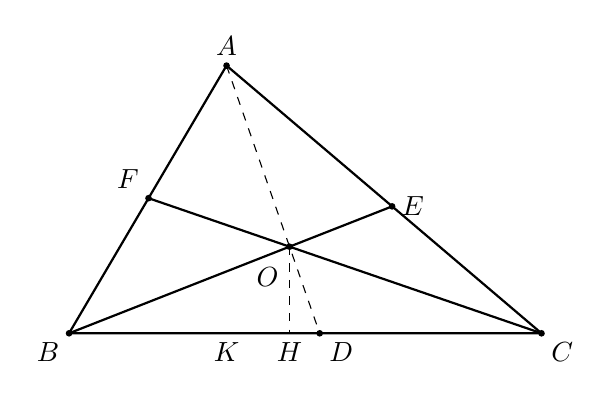
\begin{tikzpicture}[scale=1.0]
  \coordinate (A) at (2.0,3.4);
  \coordinate (B) at (0,0);
  \coordinate (C) at (6,0);
  \coordinate (O) at (2.8,1.1);
  \coordinate (D) at (3.183,0);
  \coordinate (E) at (4.103,1.612);
  \coordinate (F) at (1.009,1.716);
  \coordinate (K) at (2.0,0);
  \coordinate (H) at (2.8,0);
  \draw[thick] (A)--(B)--(C)--cycle;
  \draw[thick] (B)--(E);
  \draw[thick] (C)--(F);
  \draw[dashed] (A)--(D);
  \draw[dashed] (O)--(H);
  \fill (A) circle (1.2pt) node[above] {$A$};
  \fill (B) circle (1.2pt) node[below left] {$B$};
  \fill (C) circle (1.2pt) node[below right] {$C$};
  \fill (O) circle (1.2pt);
  \fill (D) circle (1.2pt) node[below right] {$D$};
  \fill (E) circle (1.2pt) node[right] {$E$};
  \fill (F) circle (1.2pt) node[above left] {$F$};
  \node[below] at (K) {$K$};
  \node[below] at (H) {$H$};
  \node at (2.52,0.72) {$O$};
\end{tikzpicture}
\end{center}
\nopagebreak[4]
\Needspace{5\baselineskip}
作 $\triangle ABC$ 的高 $AK$ 与 $\triangle OBC$ 的高 $OH$，$K$、$H$ 都在 $BC$ 上。$AK$ 与 $OH$ 同垂直于 $BC$，且 $A$、$O$、$D$ 共线，故 $\mathrm{Rt}\triangle AKD\sim\mathrm{Rt}\triangle OHD$，从而

\nopagebreak[4]
\[
\frac{OH}{AK}=\frac{OD}{AD}.
\]

\Needspace{5\baselineskip}
又

\nopagebreak[4]
\[
S_{\triangle OBC}=\frac12\,BC\cdot OH,
\qquad
S_{\triangle ABC}=\frac12\,BC\cdot AK,
\]

\Needspace{5\baselineskip}
所以

\nopagebreak[4]
\[
\frac{S_{\triangle OBC}}{S_{\triangle ABC}}
=\frac{\frac12\,BC\cdot OH}{\frac12\,BC\cdot AK}
=\frac{OH}{AK}
=\frac{OD}{AD}.
\]

\Needspace{5\baselineskip}
同理（$E$ 在 $BO$ 的延长线上、$F$ 在 $CO$ 的延长线上），

\nopagebreak[4]
\[
\frac{S_{\triangle OAC}}{S_{\triangle ABC}}=\frac{OE}{BE},
\qquad
\frac{S_{\triangle OAB}}{S_{\triangle ABC}}=\frac{OF}{CF}.
\]

\Needspace{5\baselineskip}
三式相加，三个小三角形的面积之和恰为 $\triangle ABC$ 的面积：

\nopagebreak[4]
\[
\frac{OD}{AD}+\frac{OE}{BE}+\frac{OF}{CF}
=\frac{S_{\triangle OBC}+S_{\triangle OAC}+S_{\triangle OAB}}{S_{\triangle ABC}}
=\frac{S_{\triangle ABC}}{S_{\triangle ABC}}=1.
\]

\gkanswer{答案：见解析版}

\end{answer}
\begin{answer}
\gksolhead{7}{}

\textbf{题目}（12 分）：

\Needspace{5\baselineskip}
设 $x$、$y$、$z$ 为三个互不相等的实数，且

\nopagebreak[4]
\[
x+\frac1y=y+\frac1z=z+\frac1x,
\]

求证：$x^2y^2z^2=1$。

\begin{gktip}
\textbf{参考题}（不计分，可以不做）
\end{gktip}

\textbf{参考题 1．} 将抛物线 $y=x^2$，直线 $x=2$ 与 $x$ 轴围成的曲边三角形，绕 $x$ 轴旋转一周形成一个旋转体，求此旋转体的体积。

\Needspace{5\baselineskip}
\textbf{参考题 2．} 求不定积分

\nopagebreak[4]
\[
\int\frac{6x^2+22x+18}{(x+1)(x+2)(x+3)}\,\mathrm dx.
\]

\Needspace{4\baselineskip}
\textbf{解析}

\Needspace{5\baselineskip}
由 $x+\dfrac1y=y+\dfrac1z$ 移项：

\nopagebreak[4]
\[
x-y=\frac1z-\frac1y=\frac{y-z}{yz},
\]

\Needspace{5\baselineskip}
$x$、$y$、$z$ 互不相等保证分母 $x-y\ne0$，即

\nopagebreak[4]
\[
yz=\frac{y-z}{x-y}.
\]

\Needspace{5\baselineskip}
同理，由 $y+\dfrac1z=z+\dfrac1x$ 得 $xz=\dfrac{z-x}{y-z}$；由 $z+\dfrac1x=x+\dfrac1y$ 得 $xy=\dfrac{x-y}{z-x}$。三式相乘：

\nopagebreak[4]
\[
yz\cdot xy\cdot zx
=\frac{y-z}{x-y}\cdot\frac{x-y}{z-x}\cdot\frac{z-x}{y-z}
=1,
\]

即 $x^2y^2z^2=1$。

\textbf{参考题 1}

\Needspace{5\baselineskip}
旋转体由曲边三角形（$0\le x\le2$，$0\le y\le x^2$）绕 $x$ 轴旋转一周得到，由旋转体体积公式

\nopagebreak[4]
\[
V=\int_0^2\pi y^2\,\mathrm dx
=\pi\int_0^2x^4\,\mathrm dx
=\pi\cdot\frac{x^5}{5}\bigg|_0^2
=\frac{32\pi}{5}.
\]

\textbf{参考题 2}

\Needspace{5\baselineskip}
记积分常数为 $C_0$，以免与待定系数 $C$ 相混。设

\nopagebreak[4]
\[
\frac{6x^2+22x+18}{(x+1)(x+2)(x+3)}
=\frac{A}{x+1}+\frac{B}{x+2}+\frac{C}{x+3},
\]

\Needspace{5\baselineskip}
去分母：

\nopagebreak[4]
\[
6x^2+22x+18=A(x+2)(x+3)+B(x+1)(x+3)+C(x+1)(x+2).
\]

\Needspace{5\baselineskip}
令 $x=-1$：$2=2A$，得 $A=1$；令 $x=-2$：$-2=-B$，得 $B=2$；令 $x=-3$：$6=2C$，得 $C=3$。于是

\nopagebreak[4]
\[
\begin{aligned}
&\int\frac{6x^2+22x+18}{(x+1)(x+2)(x+3)}\,\mathrm dx\\
&=\int\left(\frac1{x+1}+\frac2{x+2}+\frac3{x+3}\right)\mathrm dx
=\ln|x+1|+2\ln|x+2|+3\ln|x+3|+C_0,
\end{aligned}
\]

\Needspace{5\baselineskip}
合并对数：

\nopagebreak[4]
\[
\ln\left|(x+1)(x+2)^2(x+3)^3\right|+C_0.
\]

\begin{gktip}
\textbf{源注}：源解答倒数第二行印作 $\ln|x+1|+2\ln|x+2|+3\ln|x+3|+C$。

末行合并后印作 $\ln\left|(x+1)(x+2)^2(x+3)^2\right|+C$。

由 $3\ln|x+3|=\ln|x+3|^3$，末行 $(x+3)$ 的指数应与倒数第二行的系数 $3$ 相应，印作的 $2$ 系排印错误；本文按 $3$ 计算。
\end{gktip}

\gkanswer{答案：见解析版}

\end{answer}